\chapter{Model Training}\label{chapter:model_training}

\section{Data Collection}

The first step in the model training process involved preparing the dataset for training. This was achieved by recording a video of each exhibit in the museum and extracting frames from these videos. The video recordings were made using a smartphone camera, capturing various angles to ensure that users will get correct results from various angles as well. To avoid class imbalance, the number of frames to extract was determined based on the shortest video in the dataset, and the frames were then extracted at regular intervals using the \texttt{ffmpeg} tool. The extracted frames were saved in a directory structure, with each exhibit's frames stored in a separate folder under \texttt{res/frames/}. The frames were named sequentially (e.g., \texttt{frame\_01.jpg}). The corresponding code can be found in the \texttt{extract\_frames.py} script.

Additional information about each exhibit, such as the exhibit ID, title, author, and date period, was stored in a CSV file named \texttt{upm\_exhibits\_dataset.csv}. This metadata was used to label the frames during the training process (with the corresponding ID of each exhibit) and display information about the exhibits in the mobile application.

\section{Explored Solutions}

We explored two main approaches to solve the problem of exhibit recognition: embedding-based similarity search and direct classification using transfer learning.

\subsection{Embedding-based Similarity Search}

The first approach involved using a neural network to generate image embeddings. An embedding is a numeric vector representation capturing essential visual features of each image. The core idea was to pre-compute embeddings for all exhibit images in the training dataset. During inference, the neural network would generate an embedding for the user's input image, and the application would then perform a similarity search against stored embeddings to identify the closest match.

The primary advantage of this method is flexibility: adding new exhibits would not require retraining the neural network from scratch. Instead, only new embeddings would need to be generated and added to the existing collection, significantly simplifying updates.

However, this approach presented several practical challenges:

\begin{itemize}
    \item \textbf{Storage Constraints}: Our application is designed for offline usage within the museum, so image embeddings must be stored on the mobile device. Mobile devices have limited storage capacity. Storing embeddings for each exhibit --- especially as the museum collection expands --- could quickly become impractical due to the sheer volume of data.
    \item \textbf{Computational Efficiency}: Performing real-time similarity searches is computationally demanding on mobile hardware, which could lead to performance issues, especially with larger datasets.
\end{itemize}

These considerations led us to evaluate alternative methods better suited for mobile deployment and offline operation.

\subsection{Transfer Learning with Direct Classification}

The second approach, ultimately selected, was transfer learning for direct image classification. This method fine-tuned a pre-trained convolutional neural network to classify our museum exhibits. The network directly outputs probabilities corresponding to each exhibit class, eliminating the need for similarity searches.

This method offers several significant advantages:

\begin{itemize}
    \item \textbf{Efficiency and Speed}: Direct classification is computationally efficient and provides quick predictions suitable for real-time recognition on mobile devices.
    \item \textbf{Simplified Integration}: Only a single, optimized TensorFlow Lite model must be stored on the device, significantly reducing storage overhead and simplifying the integration process.
\end{itemize}

However, this approach comes with the following trade-off: when new exhibits are introduced, the model must be retrained to include these additional classes. Nonetheless, this issue can be solved by automating the training pipeline, as training times with transfer learning are typically short.

Considering these factors, direct classification using transfer learning was selected as the most suitable solution due to its balance between accuracy, performance, storage efficiency, and ease of integration.

\section{Model Selection and Setup}

As already mentioned, transfer learning was employed to adapt the pre-trained model to our task of classifying museum exhibits. This approach leverages the general features learned from pre-training and fine-tunes the chosen model to recognize the unique characteristics of the specific data. More information on transfer learning can be found in Section~\ref{section:transfer_learning}.

For our task, the MobileNetV2 architecture was selected as the base model. MobileNetV2 is a lightweight convolutional neural network specifically designed for mobile applications. It balances efficiency and accuracy, making it ideal for real-time image classification tasks on resource-constrained devices like smartphones. Further details on MobileNetV2 can be found in Section~\ref{section:mobilenet}.

The transfer learning setup involved the following steps:

\begin{enumerate}
   \item \textbf{Freezing Pre-trained Layers:} The pre-trained MobileNetV2 model was loaded with its convolutional base set to non-trainable. By freezing the early layers, the model retained its ability to extract general features learned from ImageNet, for example, detect edges, textures, and shapes.
   
   \item \textbf{Adding Custom Layers:} Custom layers were added on top of the frozen layers to adapt the model to our dataset. These included:
   \begin{itemize}
       \item \textbf{Global Average Pooling:} To reduce spatial dimensions of feature maps to a single vector per feature map, summarizing the important information.
       \item \textbf{Dense Layer:} A fully connected layer with 1024 units and ReLU activation to learn complex feature combinations relevant for exhibit classification.
       \item \textbf{Dropout Layer:} Included with a rate of 0.1 to prevent overfitting by randomly setting a fraction of input units to zero during training.
       \item \textbf{Output Layer:} A dense layer with softmax activation, where the number of units corresponds to the number of exhibit classes. This layer outputs predicted probabilities for each class.
   \end{itemize}
\end{enumerate}

\section{Training Process}

In the beginning, it is important to note that many aspects of training a neural network --- such as model architecture, learning rates, batch size, or number of epochs --- are typically determined through experimentation. While there are commonly accepted starting points (e.g., using a batch size of 16 or 32, or the Adam optimizer with a standard learning rate), there is no one-size-fits-all configuration. Each dataset and task is different, and therefore requires iterative testing and tuning to find the combination of parameters that gives the best performance. In this project, several choices were made based on such experimentation.

Also, as part of the experimentation process, the training process was divided into two main phases: initial training, in which only the custom layers were trained, and additional fine-tuning, where some of the pre-trained layers were unfrozen to allow for further learning on the museum exhibit dataset.

\subsection{Initial Training and Evaluation}

During the initial training phase, the custom layers added on top of the pre-trained base were trained on the museum exhibit dataset. The training setup and details are as follows:

\begin{itemize}
   \item \textbf{Optimizer:} Adam optimizer, used with the default learning rate of \(1 \times 10^{-3}\).
   \item \textbf{Loss Function:} Categorical cross-entropy, suitable for multi-class classification.
   \item \textbf{Metrics:} Accuracy, showing how often the predictions matched actual labels.
   \item \textbf{Epochs:} 20 epochs, determined by monitoring the model's performance on the validation set (will be covered later in this section).
   \item \textbf{Batch Size:} Batch size of 16, which is a common choice.
   \item \textbf{Validation:} 20\% of the data was kept aside to monitor how well the model performed on unseen data.
\end{itemize}

This setup gives us 0.945 accuracy on the validation set after 20 epochs of training, and it can be seen in Figure~\ref{fig:initial_training} that there is no significant improvement in accuracy after the 10th epoch, indicating that the model has likely converged (same results were obtained when training for 40 epochs).

\begin{figure}[h]
    \centering
    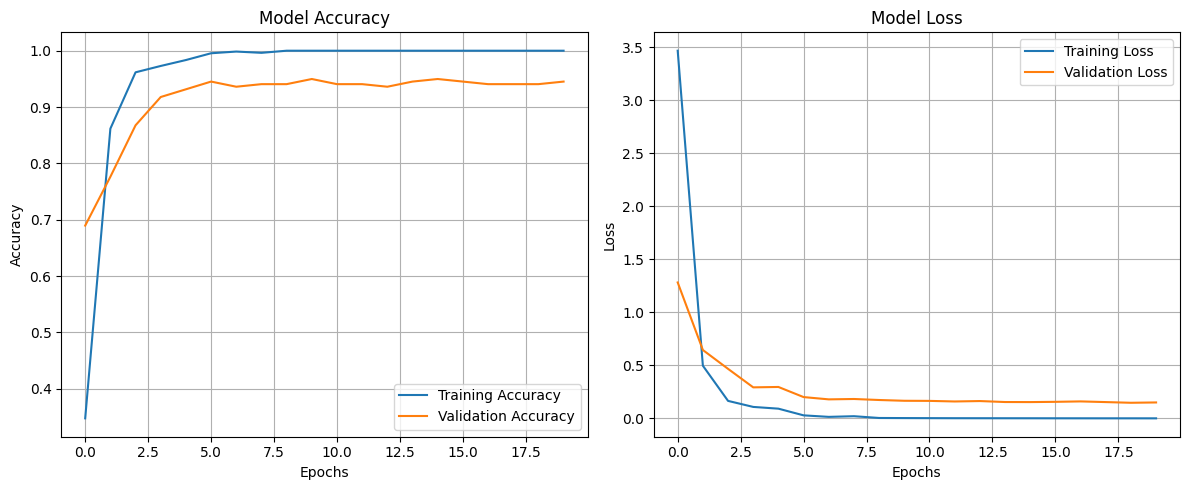
\includegraphics[width=1.0\textwidth]{img/initial-training.png}
    \caption{Training and validation accuracy and loss during the initial training phase.}\label{fig:initial_training}
\end{figure}

While the initial results are already quite good, further fine-tuning might improve the model's performance by adjusting some of the pre-trained layers to better fit the new dataset.

\subsection{Additional Fine-tuning and Evaluation}

After the initial training, the model was trained further with some of the pre-trained layers unfrozen. This optional step can improve the model's performance by adjusting some of the pre-trained layers to better fit the new dataset.

The number of layers to unfreeze depends on how similar the new dataset is to the dataset the model was initially trained on (ImageNet) and on the size of the new dataset. If the new data is very different, unfreezing more layers can help the model adjust better. As for the size, if the new dataset is small, unfreezing too many layers can lead to overfitting. A common strategy is to unfreeze the last few dozen layers. For example, the official TensorFlow tutorial~\cite{tensorflow_transfer_learning} demonstrates unfreezing MobileNetV2 from about layer 100 onward (out of 154) --- i.e., fine-tuning the last 54 layers (around the top one-third of the network). It is also recommended to fine-tune with a lower learning rate, since large weight updates on pre-trained layers can disrupt the learned features, leading to worse performance.

We experimented with unfreezing the last 14, 24, and 34 layers of the pre-trained model. During fine-tuning, the learning rate was lowered to \(1 \times 10^{-5}\) to avoid significant changes to already learned features. Fine-tuning continued for another 20 epochs after the initial training. The best results were achieved when unfreezing the last 34 layers (meaning that the first 120 layers were frozen), which resulted in a validation accuracy of 0.959 after fine-tuning. This gives us a 1.4\% improvement over the initial training phase, which is a slight improvement considering that the model was already performing well. The results of the fine-tuning phase can be seen in Figure~\ref{fig:fine_tuning}.

\begin{figure}[h]
    \centering
    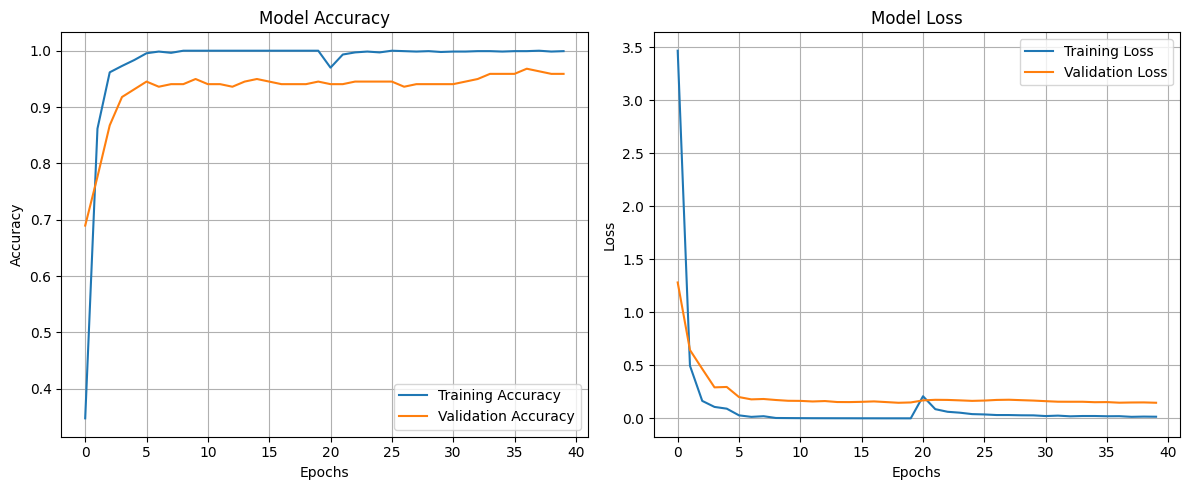
\includegraphics[width=1.0\textwidth]{img/fine-tuning.png}
    \caption{Training and validation accuracy and loss during the fine-tuning phase.}\label{fig:fine_tuning}
\end{figure}

\section{Other Experiments}

Several other experiments were conducted during the training process to explore different configurations and their impact on model performance. These included:

\begin{itemize}
    \item \textbf{Batch Sizes:} Different batch sizes (8, 16, and 32) were tested, which did not affect the model's performance. A batch size of 16 was chosen as a good compromise between training speed and memory usage.
    \item \textbf{Data Augmentation:} Various data augmentation techniques were applied, such as rotation, width and height shifts, and zooming. However, these did not improve the model's performance; instead, they increased training time. Therefore, no data augmentation was used in the final model.
    \item \textbf{More Layers}: Additional dense layers were added to the model, which increased the model's training time but did not improve the accuracy.
    \item \textbf{Increased Dropout Rate:} The dropout rate was increased to 0.5, which resulted in a lower validation accuracy.
\end{itemize}

Thus, the final model configuration was chosen based on the best results from these experiments, which included a batch size of 16, no data augmentation, one dense layer, and a dropout rate of 0.1.

In the following section, we will analyze the misclassifications made by the model during the validation phase to better understand its performance and identify potential areas for improvement.

\section{Analysis of Misclassifications}

To better understand the model's performance, we analyzed the misclassifications made during the validation phase. This analysis helps identify patterns in errors and provides insights into potential improvements.

Of 219 images in the validation set, nine were misclassified, resulting in a validation accuracy of 0.959. In Table~\ref{tab:misclassifications}, we can see the misclassified images along with their actual and predicted labels. Actual labels are shown in the second column, while the model's predictions are in the third column.

\begin{table}[h]
    \centering
    \begin{tabular}{lcc}
        \toprule
        \textbf{Filepath} & \textbf{True label} & \textbf{Pred.\ label} \\
        \midrule
        \texttt{res/frames/85/frame\_01.jpg}  & 85  & 87  \\
        \texttt{res/frames/90/frame\_01.jpg}  & 90  & 88  \\
        \texttt{res/frames/102/frame\_01.jpg} & 102 & 175 \\
        \texttt{res/frames/105/frame\_10.jpg} & 105 & 103 \\
        \texttt{res/frames/110/frame\_01.jpg} & 110 & 111 \\
        \texttt{res/frames/115/frame\_10.jpg} & 115 & 111 \\
        \texttt{res/frames/117/frame\_01.jpg} & 117 & 118 \\
        \texttt{res/frames/138/frame\_01.jpg} & 138 & 137 \\
        \texttt{res/frames/173/frame\_01.jpg} & 173 & 171 \\
        \bottomrule
    \end{tabular}
    
    \caption{Misclassified validation images with their true and predicted labels.}\label{tab:misclassifications}
\end{table}

If we look at the actual labels and predicted labels, we can see that most of them are very close to each other (85--87, 90--88, 105--103, and so on). Exhibits were recorded and labeled one after another, so the exhibits whose labels are close to each other are likely to be visually similar, because they are from the same collection or share the same style or theme. Moreover, some frames from video recordings contain multiple exhibits, which can lead to confusion for the model. For example, the image with label 138 contains two exhibits (with a true label 138 and our predicted label 137) in the same frame, which makes it difficult for the model to distinguish between them. Figure~\ref{fig:misclassifications_examples1} and Figure~\ref{fig:misclassifications_examples2} show some examples of misclassified images with their true labels and model predictions.

This leads us to the conclusion that the model is performing well enough for the exhibits that are visually distinct, but it might struggle with similar-looking exhibits or those captured in the same frame. In order to address this issue, our application will provide the user with the top-recognized exhibit as the main prediction, and up to four alternatives for user selection ordered by confidence level. This approach will help improve the user experience and ensure that users can find the information they are looking for, even if the model makes a mistake.

\begin{figure}[h]
    \centering

    \begin{subfigure}[b]{0.4\textwidth}
        \centering
        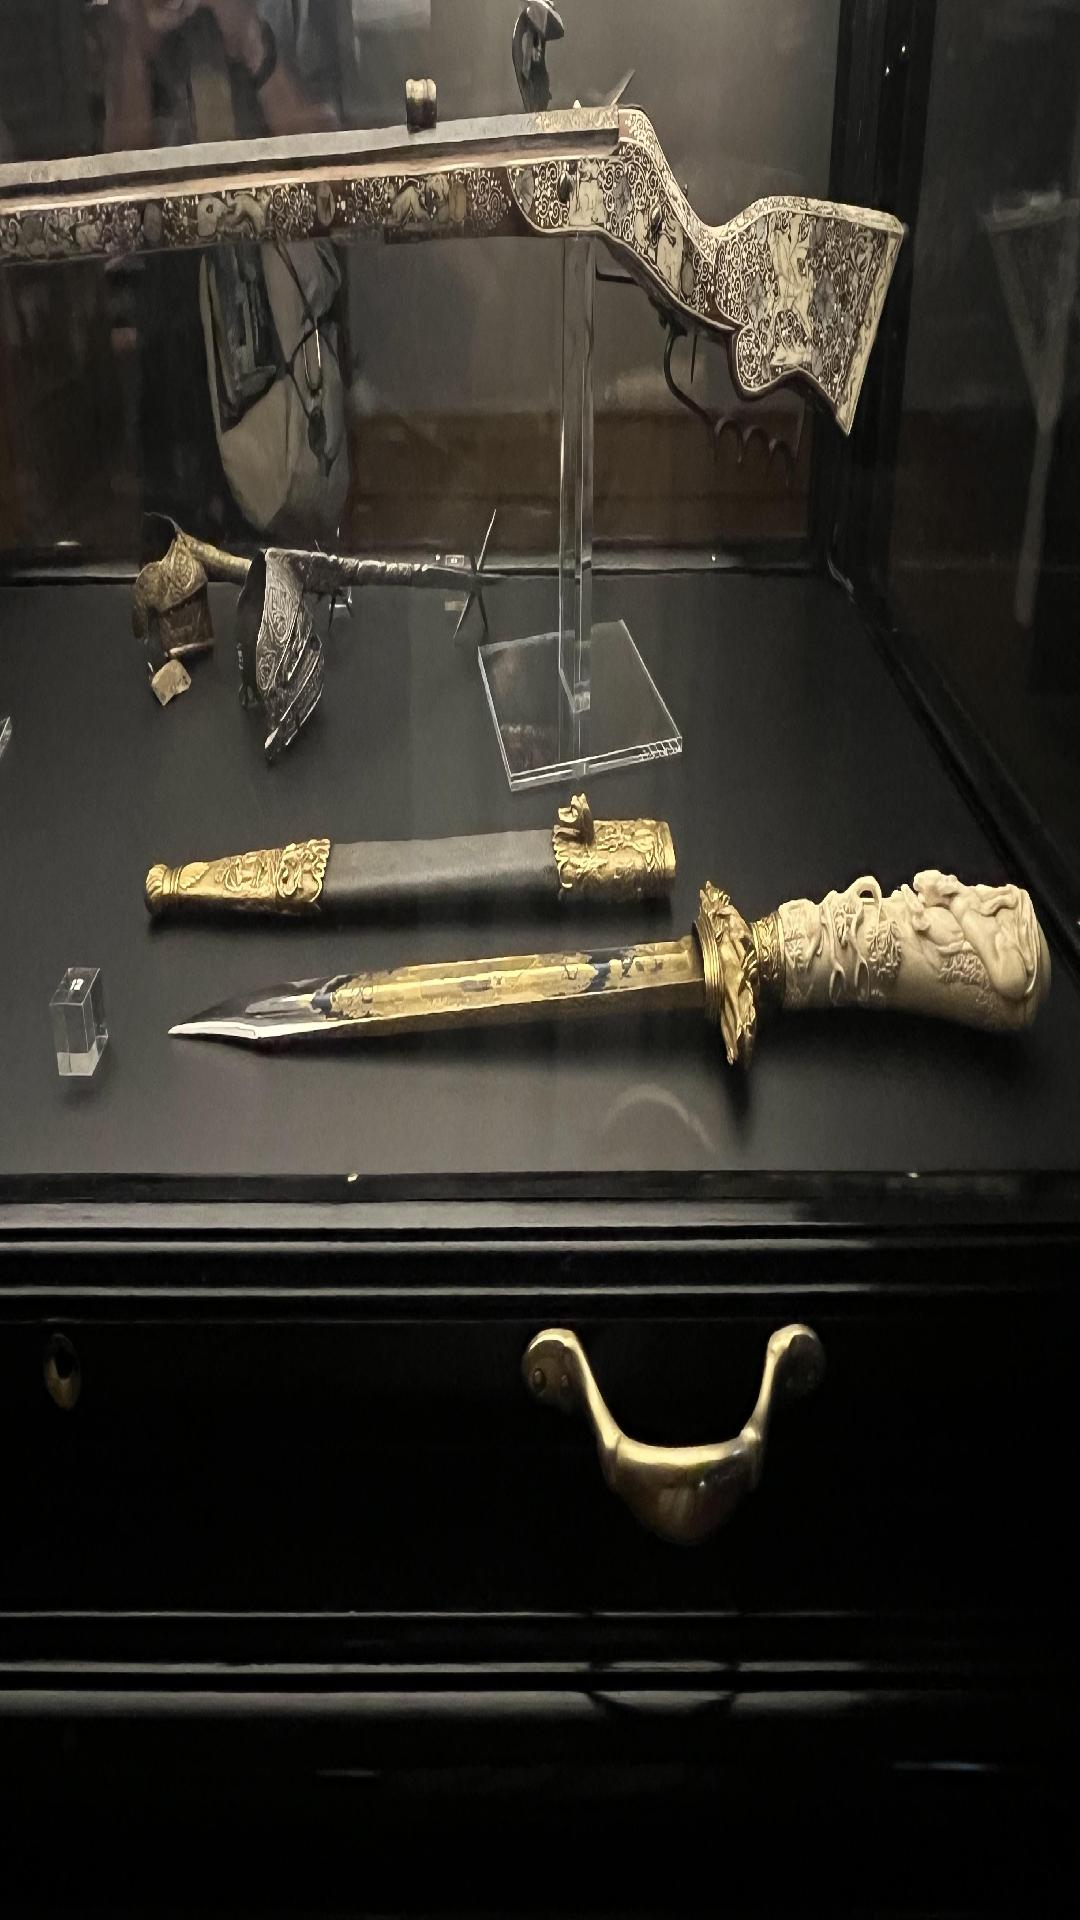
\includegraphics[width=\textwidth]{img/138.jpg}
        \caption{Input image with true label 138.}
    \end{subfigure}
    \hfill
    \begin{subfigure}[b]{0.4\textwidth}
        \centering
        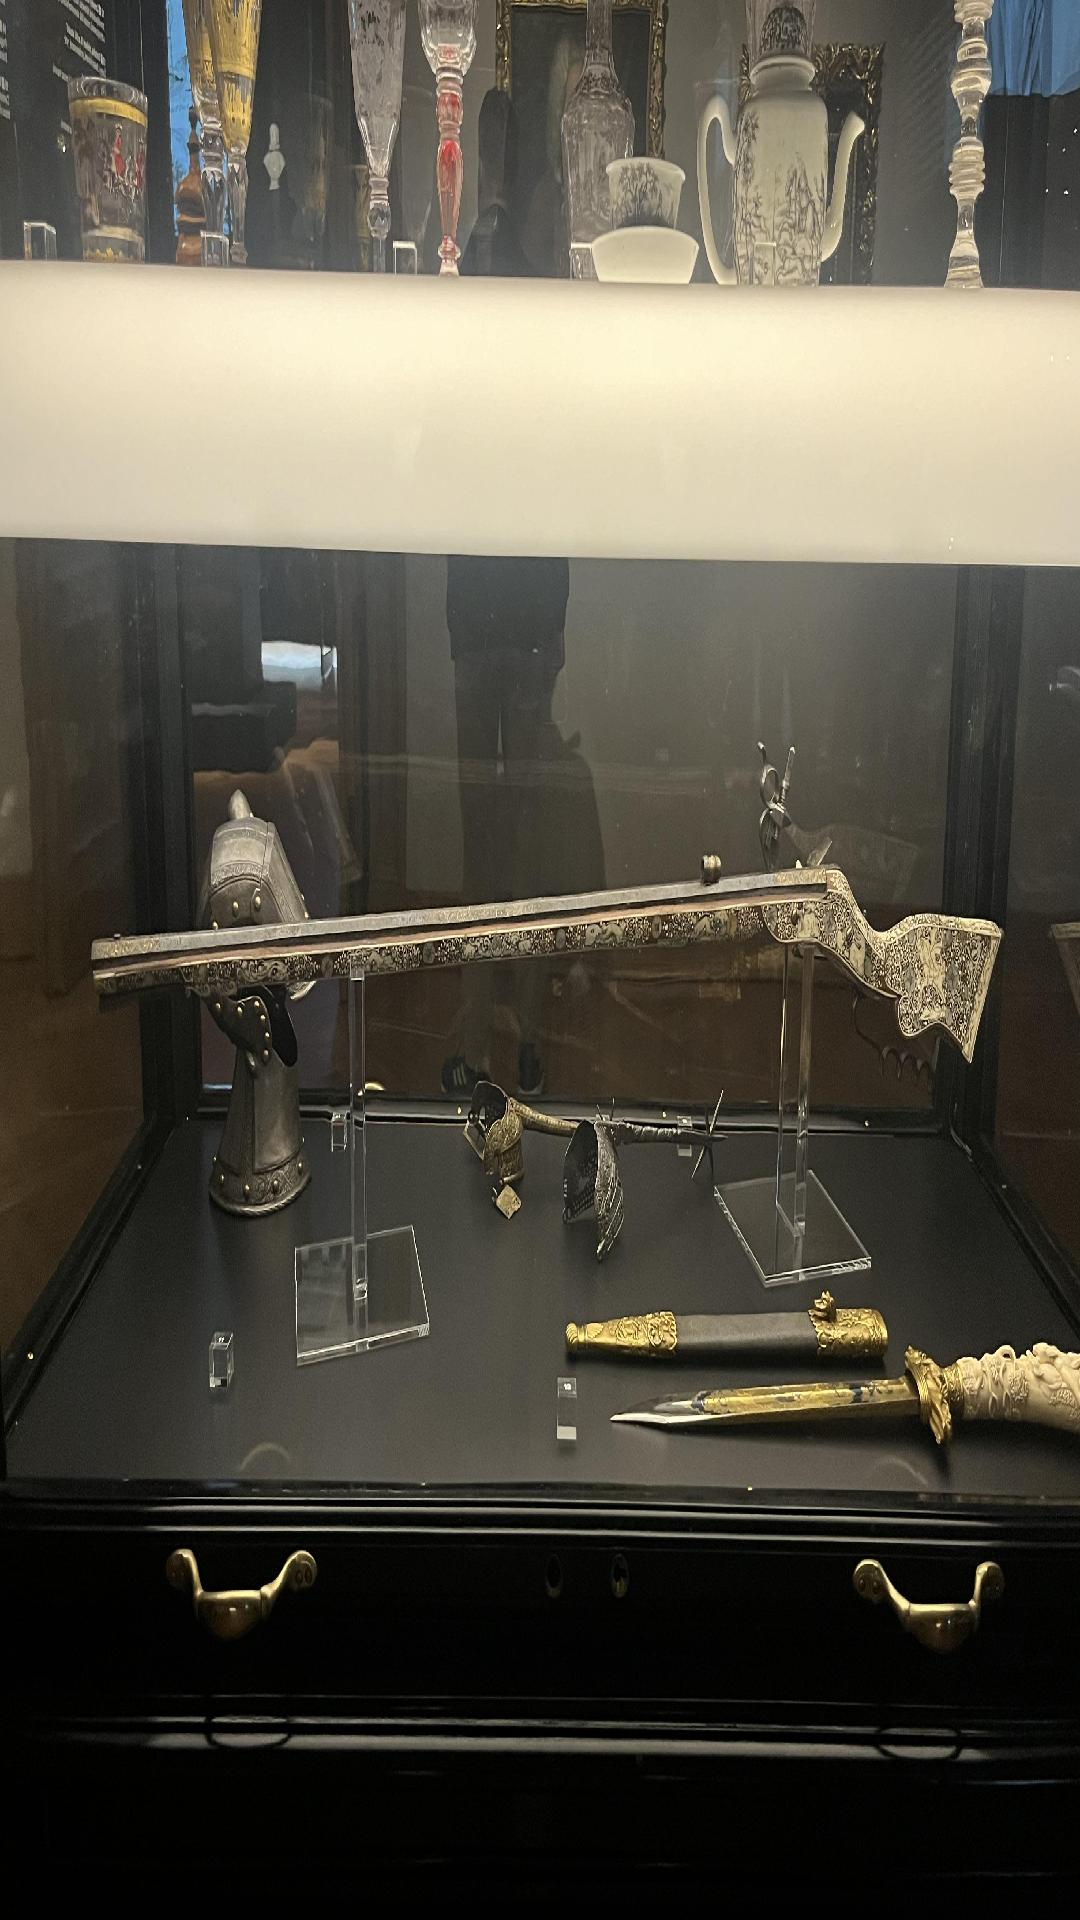
\includegraphics[width=\textwidth]{img/137.jpg}
        \caption{Image of the predicted label 137.}
    \end{subfigure}

    \vspace{1em}

    \begin{subfigure}[b]{0.4\textwidth}
        \centering
        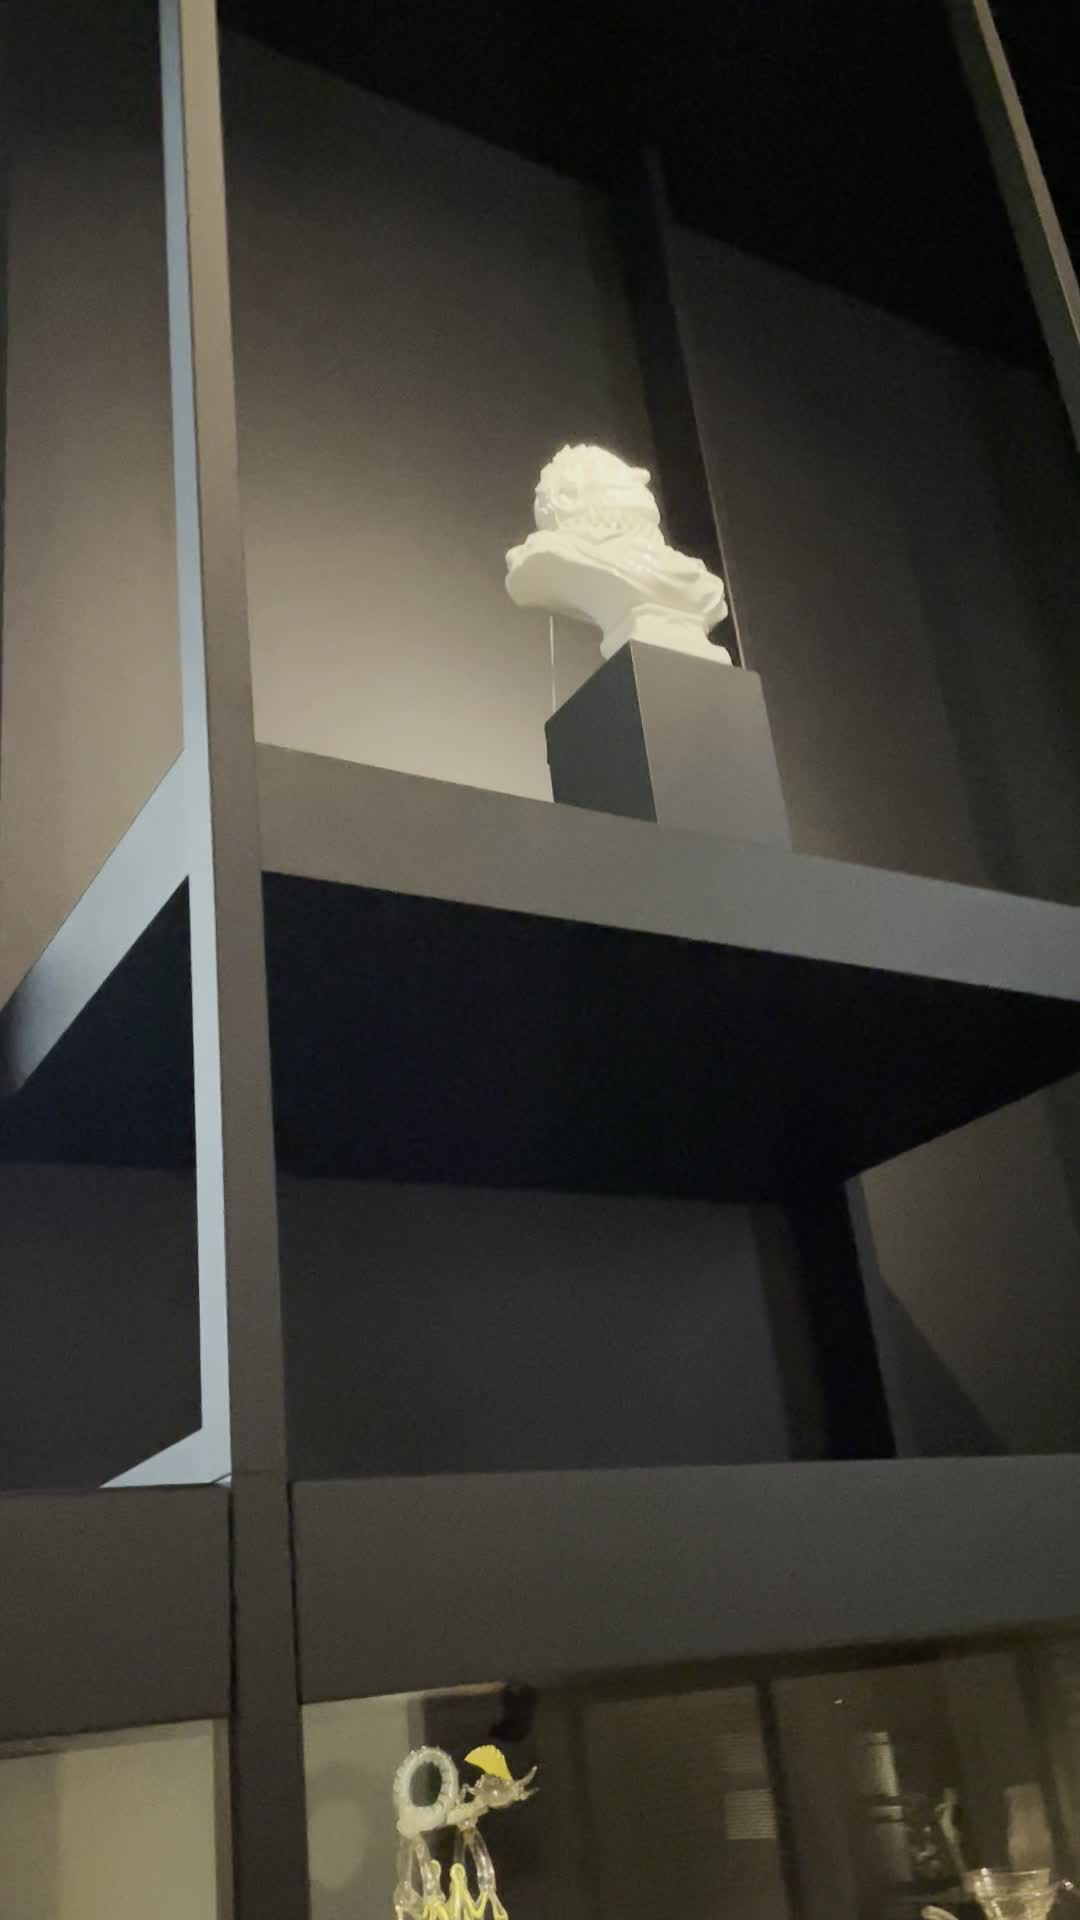
\includegraphics[width=\textwidth]{img/85.jpg}
        \caption{Input image with true label 85.}
    \end{subfigure}
    \hfill
    \begin{subfigure}[b]{0.4\textwidth}
        \centering
        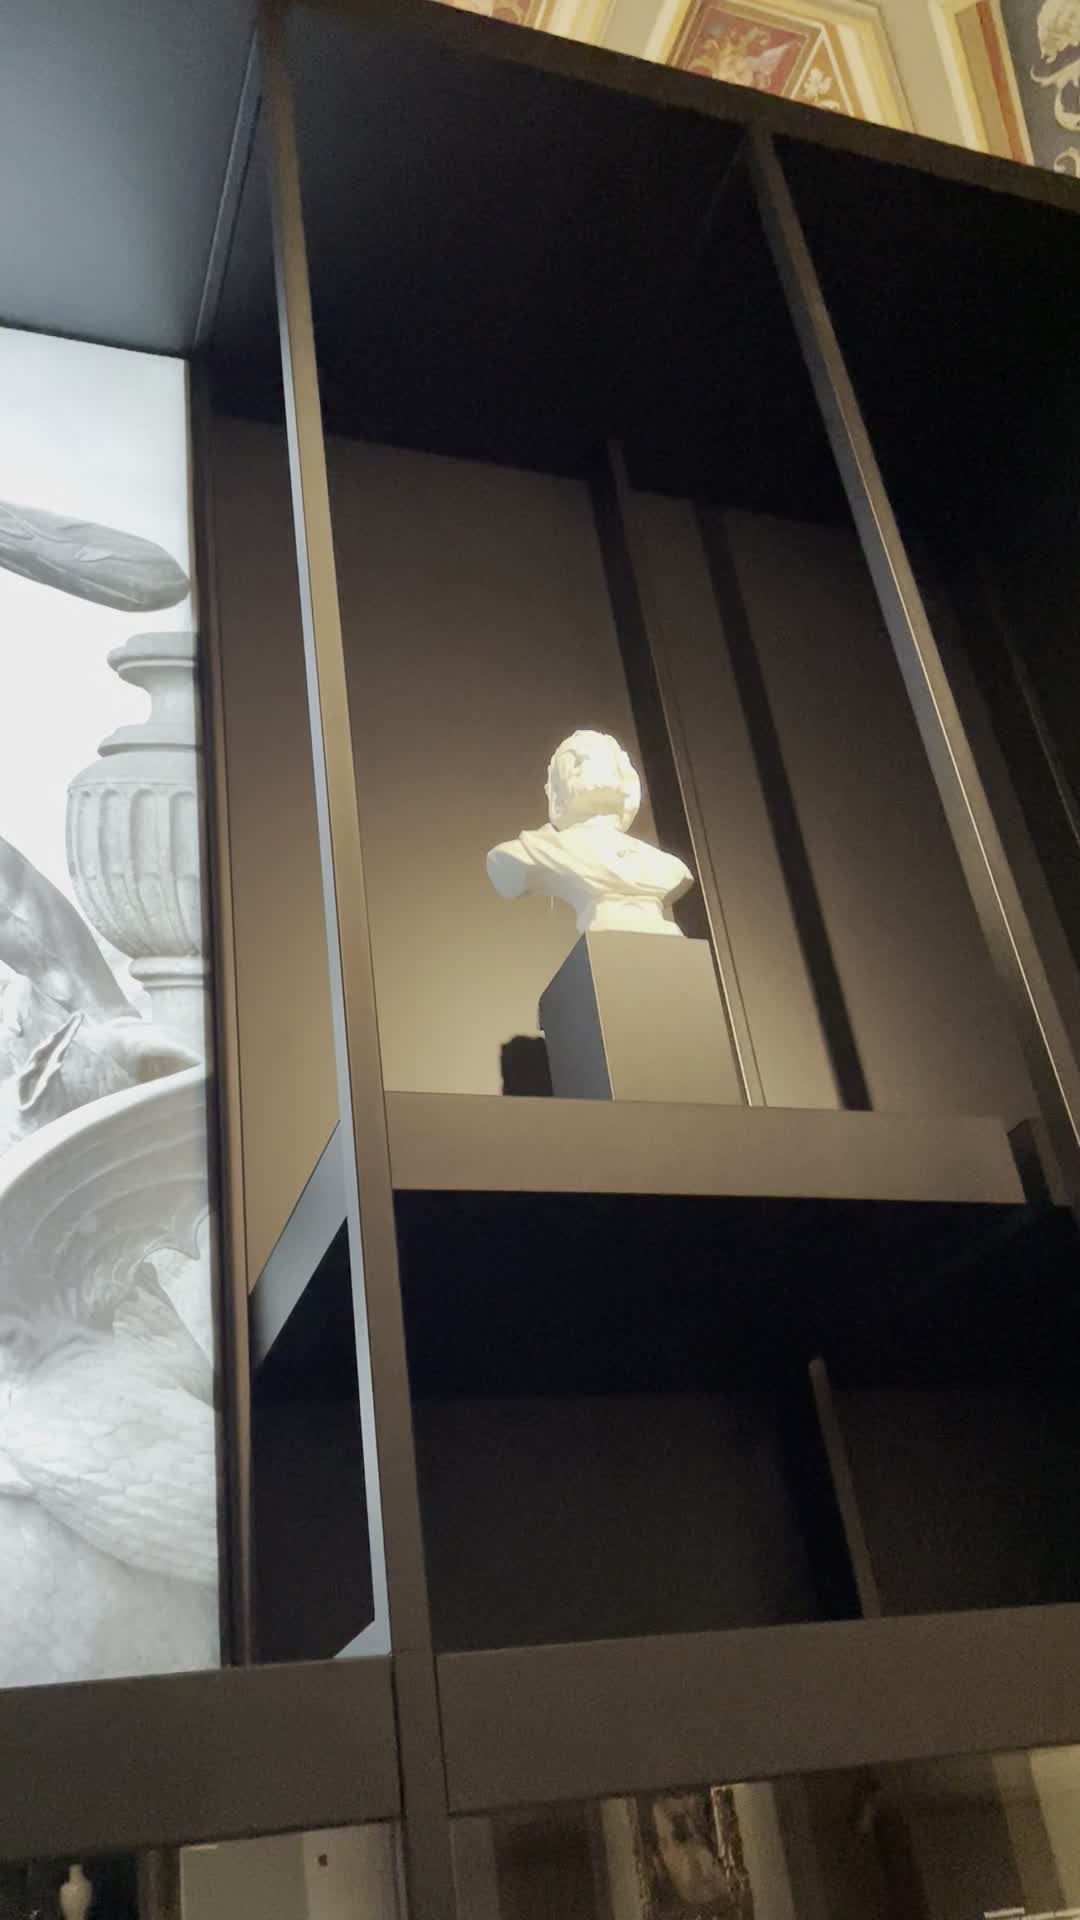
\includegraphics[width=\textwidth]{img/87.jpg}
        \caption{Image of the predicted label 87.}
    \end{subfigure}

    \caption{Misclassified images with their true labels and model predictions (1/2).}\label{fig:misclassifications_examples1}
\end{figure}

\begin{figure}[h]
    \centering

    \begin{subfigure}[b]{0.4\textwidth}
        \centering
        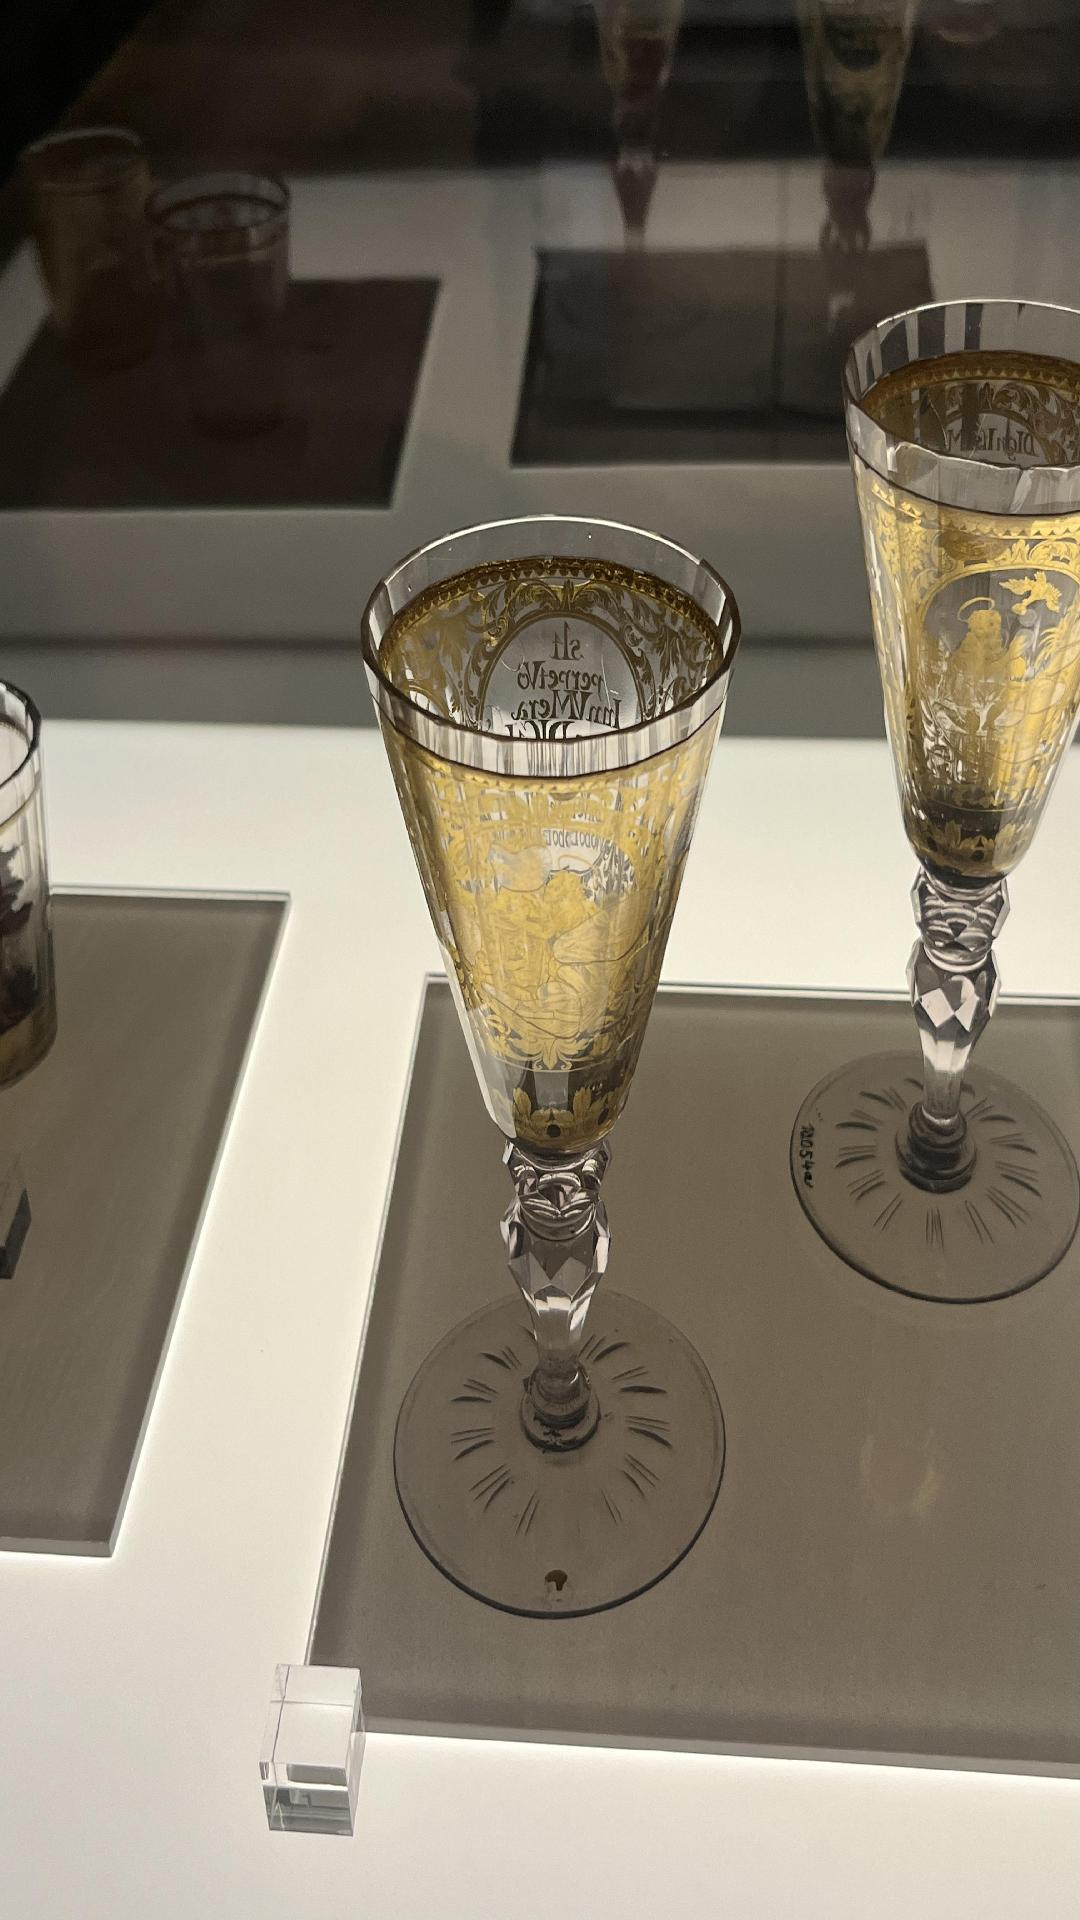
\includegraphics[width=\textwidth]{img/117.jpg}
        \caption{Input image with true label 117.}
    \end{subfigure}
    \hfill
    \begin{subfigure}[b]{0.4\textwidth}
        \centering
        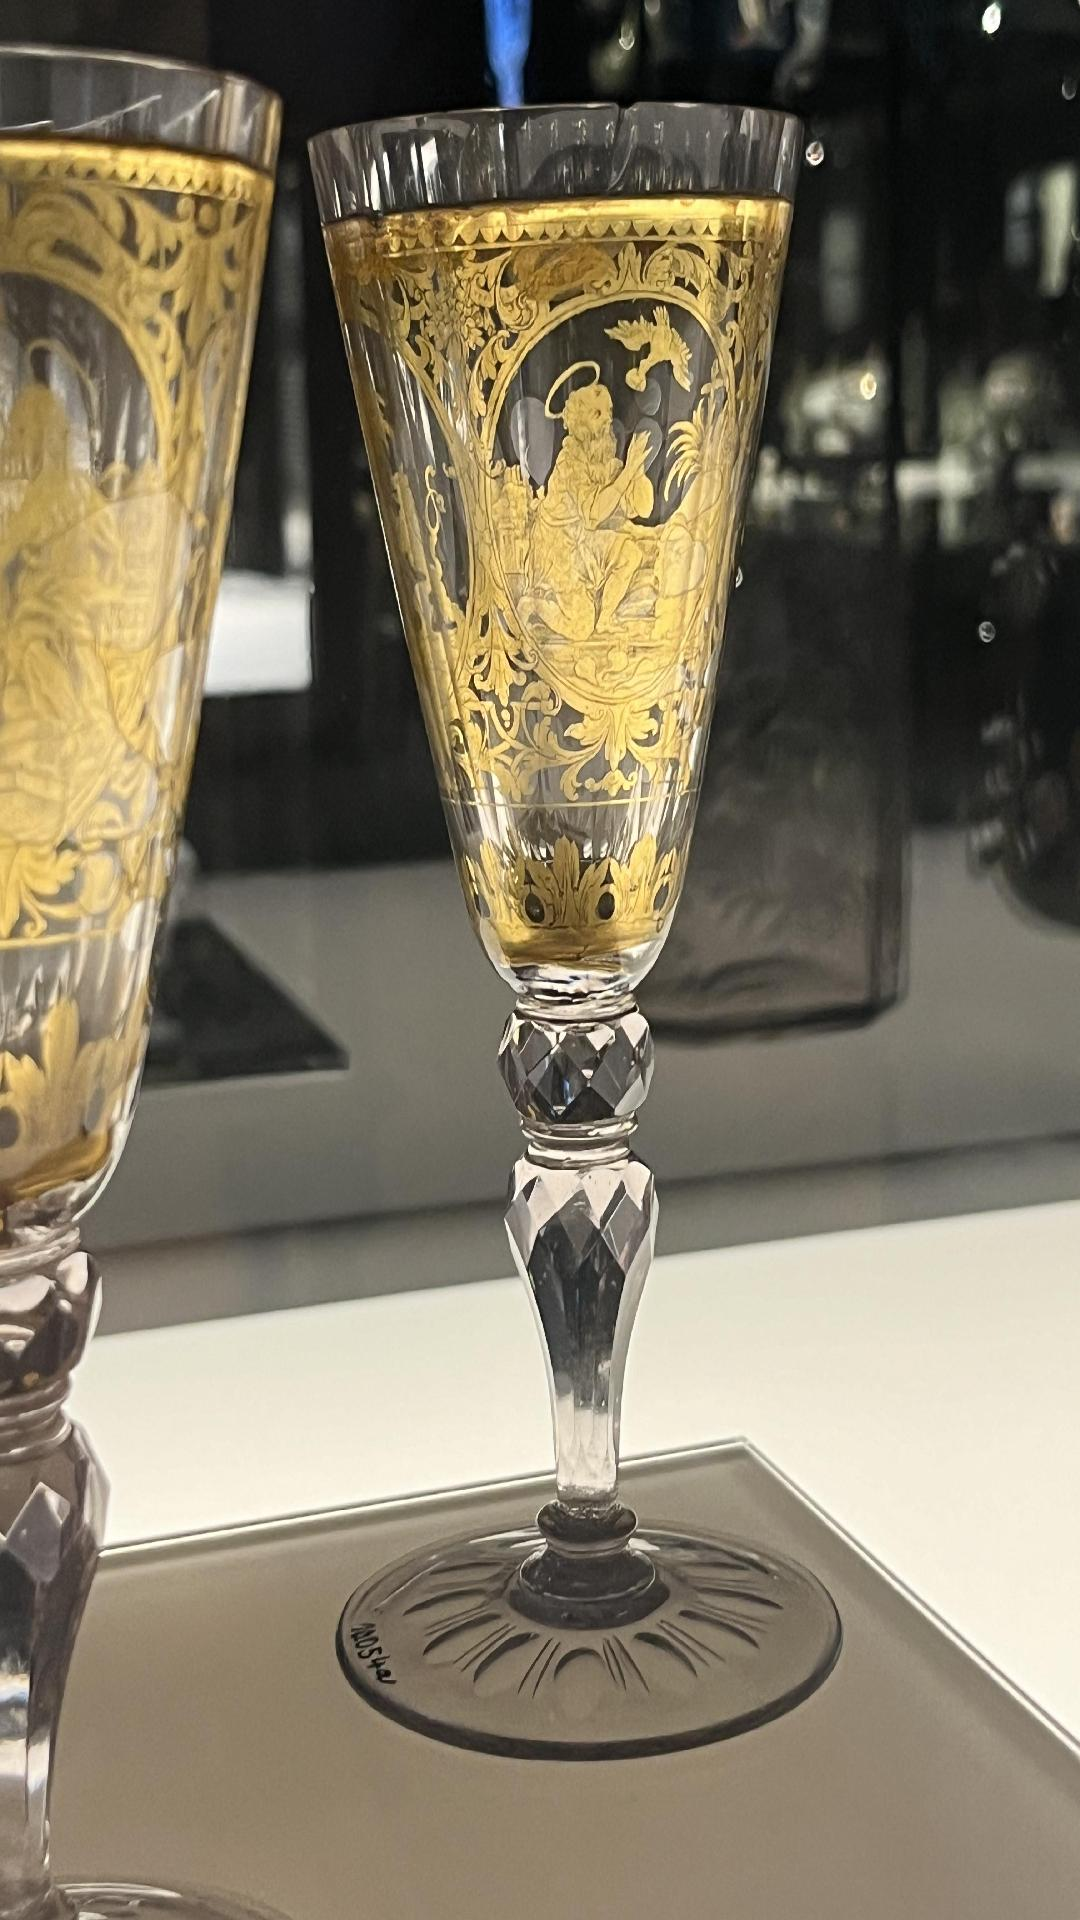
\includegraphics[width=\textwidth]{img/118.jpg}
        \caption{Image of the predicted label 118.}
    \end{subfigure}

    \vspace{1em}

    \begin{subfigure}[b]{0.4\textwidth}
        \centering
        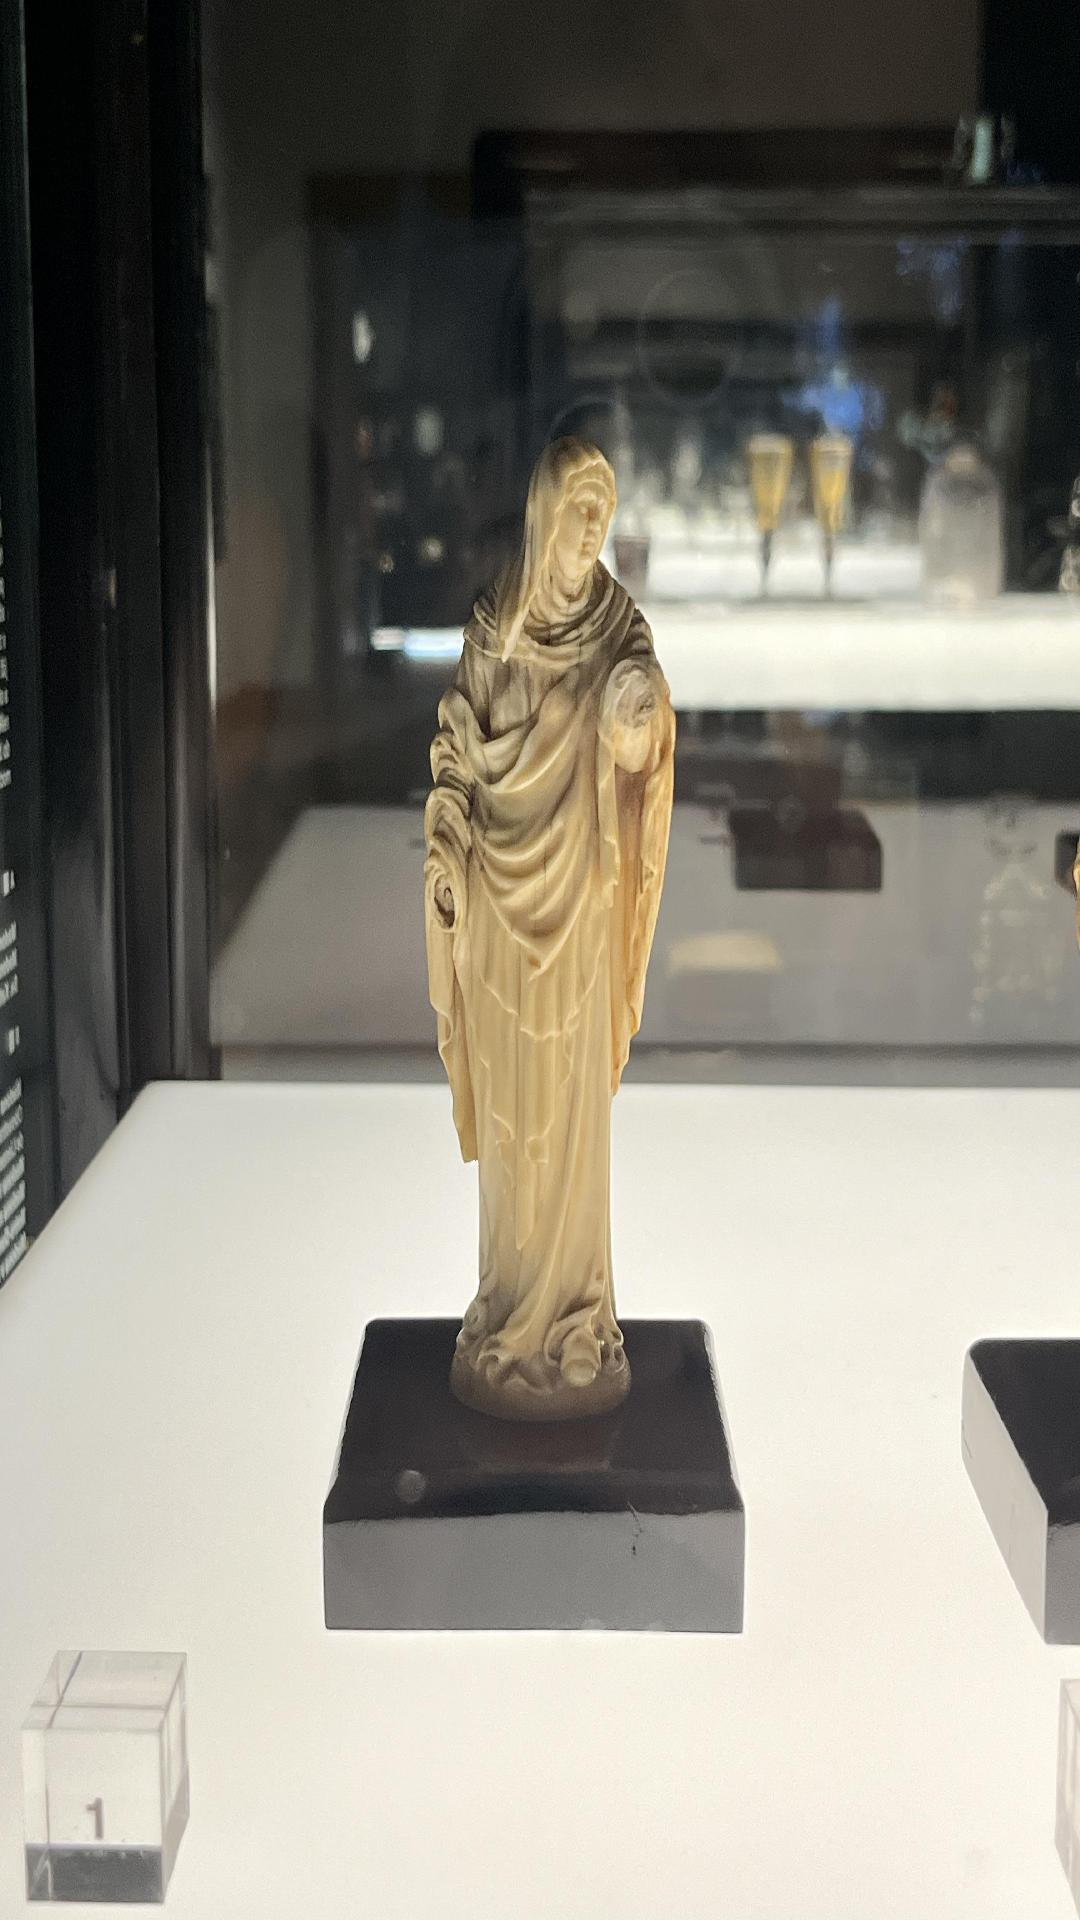
\includegraphics[width=\textwidth]{img/110.jpg}
        \caption{Input image with true label 110.}
    \end{subfigure}
    \hfill
    \begin{subfigure}[b]{0.4\textwidth}
        \centering
        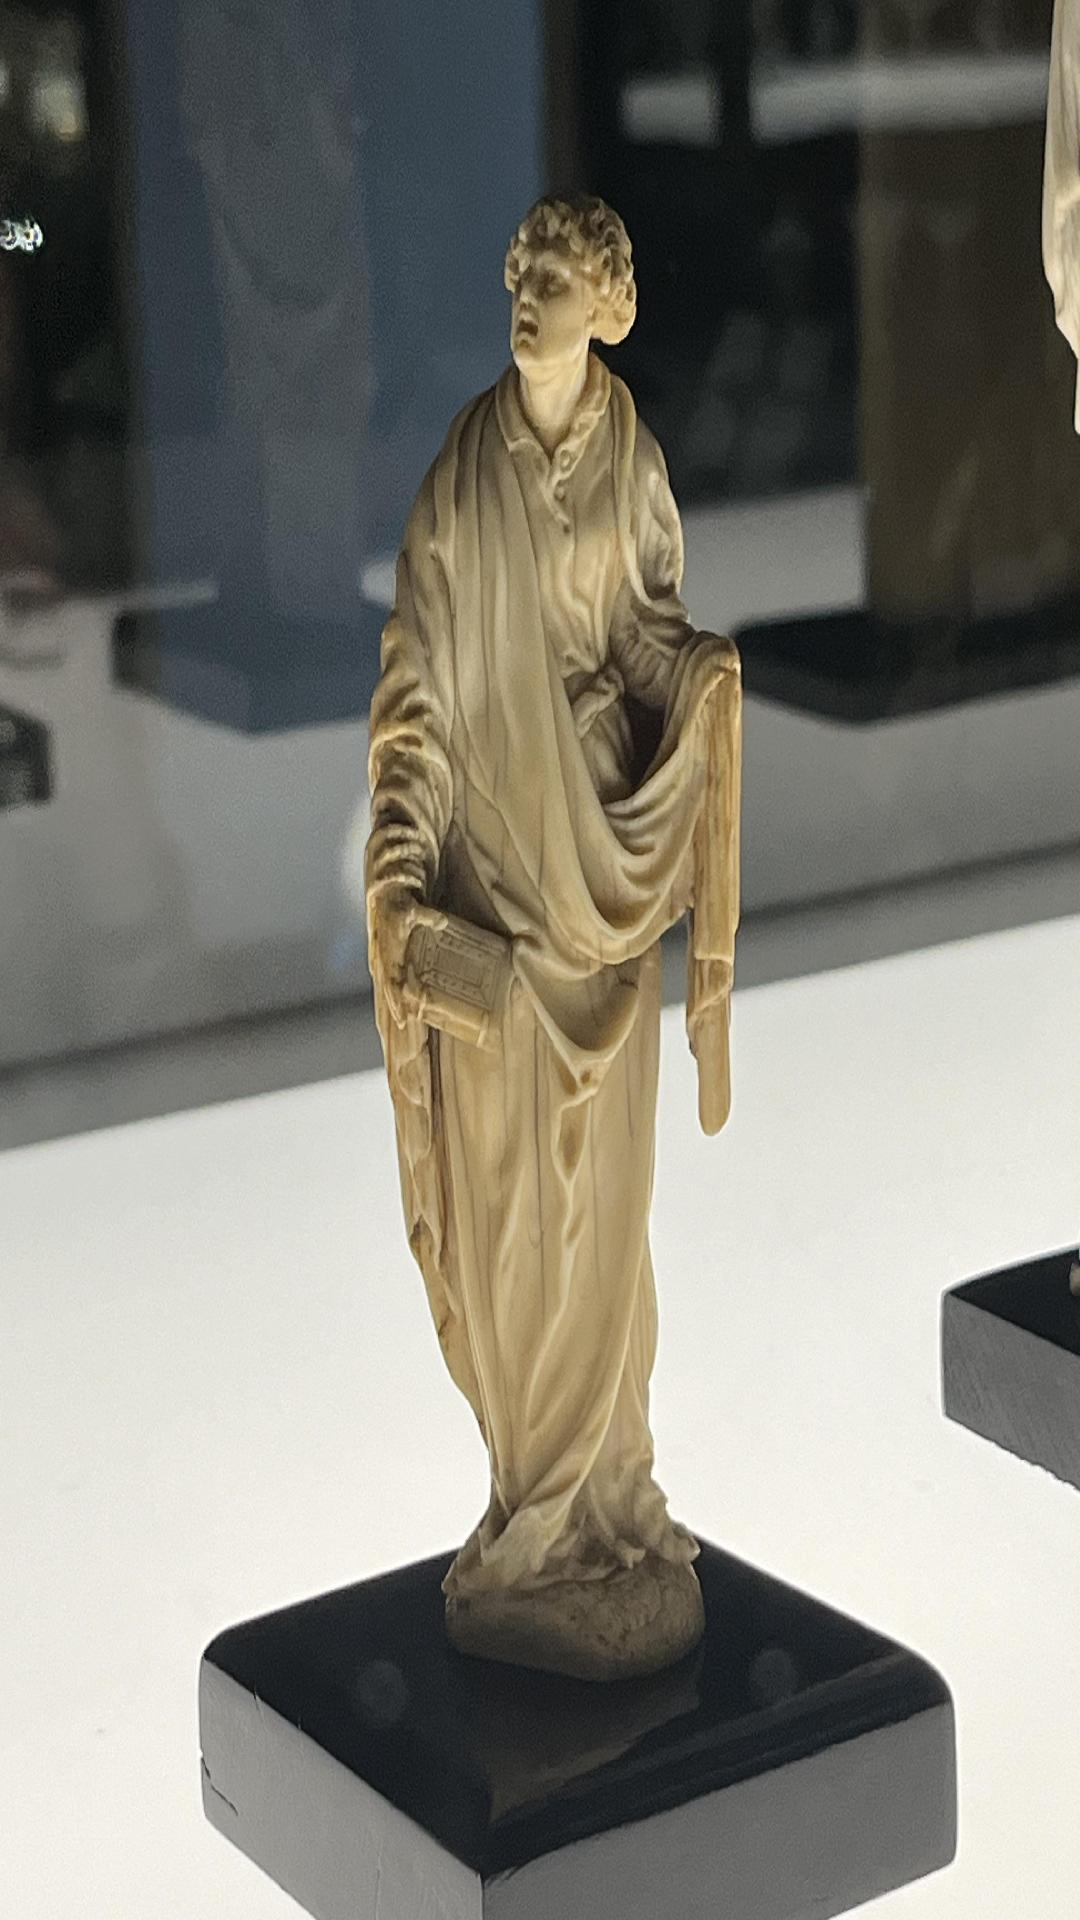
\includegraphics[width=\textwidth]{img/111.jpg}
        \caption{Image of the predicted label 111.}
    \end{subfigure}

    \caption{Misclassified images with their true labels and model predictions (2/2).}\label{fig:misclassifications_examples2}
\end{figure}


\section{TensorFlow Lite}

The trained model was converted to TensorFlow Lite format to use the model on mobile devices. TensorFlow Lite (now known as LiteRT~\cite{tensorflow_lite}) reduces model size and complexity, allowing it to run quickly on smartphones. The conversion was done using TensorFlow's built-in converter (TFLiteConverter), compressing the model without losing much accuracy.

\section{Conclusion}

In this chapter, we have described the process of training a machine learning model to recognize museum exhibits. We explored different approaches, ultimately selecting transfer learning with the MobileNetV2 architecture. The model was trained on a dataset of frames extracted from video recordings of exhibits, achieving a validation accuracy of 0.959 after fine-tuning.

We also analyzed the misclassifications made by the model, identifying patterns in errors and providing insights into addressing these errors. The model was converted to TensorFlow Lite format for deployment on mobile devices, ensuring efficient performance in real-time exhibit recognition.